%%%%%%%%%%%%%%%%%%%%%%%%%%%%%%%%%%%%%%%%%%%%%%%%%%%%%%%%%%%%%%%%%%%%%%%%%%%%%%%%
\chapter{Machine Learning\label{chap:ML}}
%%%%%%%%%%%%%%%%%%%%%%%%%%%%%%%%%%%%%%%%%%%%%%%%%%%%%%%%%%%%%%%%%%%%%%%%%%%%%%%%

% 2) A feedforward neural network, as formally defined in the article concerning feedforward neural networks, whose parameters are collectively denoted θ\thetaθ. In backpropagation, the parameters of primary interest are wijkw_{ij}^kwijk​, the weight between node jjj in layer lkl_klk​ and node iii in layer lk−1l_{k-1}lk−1​, and bikb_i^kbik​, the bias for node iii in layer lkl_klk​. There are no connections between nodes in the same layer and layers are fully connected.
% 3) An error function, E(X,θ)E(X, \theta)E(X,θ), which defines the error between the desired output yi⃗\vec{y_i}yi
%  and the calculated output yi⃗^\hat{\vec{y_i}}yi​​^​ of the neural network on input xi⃗\vec{x_i}xi​​ for a set of input-output pairs (xi⃗,yi⃗)∈X\big(\vec{x_i}, \vec{y_i}\big) \in X(xi​​,yi​​)∈X and a particular value of the parameters θ\thetaθ.

Machine learning, often described as a proper subset of artificial
intelligence \cite{Goodfellow-et-al-2016}, and is the field in computer science
which deals with the improvement of algorithms through experience and the use of
data \cite{Mitchell97}. Our daily lives exhibit wide applications of intelligent
software to automate routine labour, understand speech or images, assist in
diagnoses in medicine and support basic scientific research. This field as a
whole is relatively young, having been coined in 1959 by Arthur Samuel
\cite{5392560}, however little progress in reaching human-comparable learning
was achieved until the advent of deep learning, termed by Rina Dechter in 1986
\cite{Rina1986}. Even then, human-like recognition of real-world images was not
achieved until ImageNet was created in 2009 \cite{5206848}, which is often
considered as the catalyst for the AI boom of the 21st century
\cite{hardy_2016}.

\begin{figure}[htp!]
    \centering
    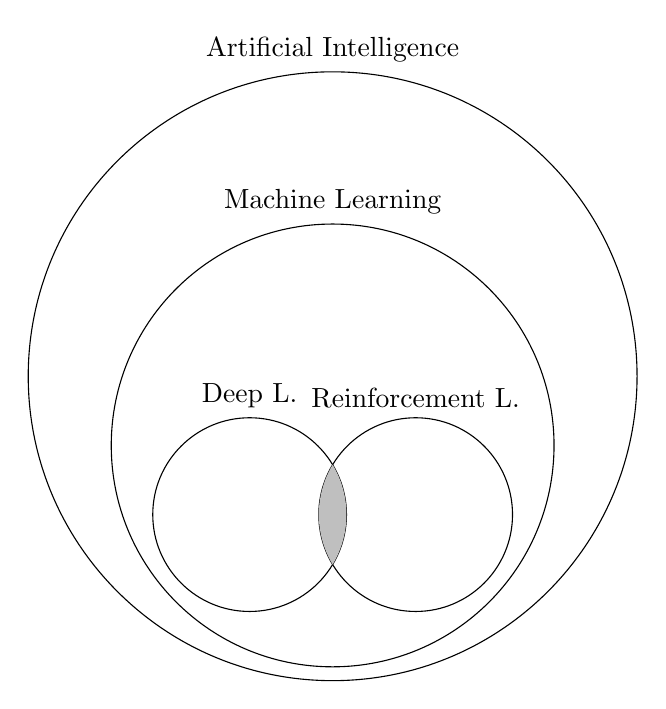
\begin{tikzpicture}

    % Circle with label
    \node[draw,
        circle,
        minimum size =22em,
        label=Artificial Intelligence] (ai_circ) at (0,0){};

    % Circle with label
    \node[draw,
        circle,
        minimum size =16em,
        label=Machine Learning] (ml_circ) at (0,-2.5em){};

    % Circle with label
    \node[draw,
        circle,
        minimum size =7em,
        label=Deep L.] (dl_circ) at (-3em,-5em){};

    \node[draw,
        circle,
        minimum size =7em,
        label=Reinforcement L.] (rl_circ) at (3em,-5em){};


    % Intersection
    \begin{scope}
        \clip (-3em,-5em) circle(3.5em);
        \clip (3em,-5em) circle(3.5em);
        \fill[gray!50](3em,-5em) circle(3.5em);
    \end{scope}

\end{tikzpicture}
    \caption{
        The relationship between the fields of Artificial Intelligence,
        Machine Learning, Deep Learning and Reinforcement Learning.
    }
    \label{fig:al-ml-dl}
\end{figure}


\newpage


\section{Machine Learning Basics}
%%%%%%%%%%%%%%%%%%%%%%%%%%%%%%%%%%%%%%%%%%%%%%%%%%%%%%%%%%%%%%%%%%%%%%%%%%%%%%%%
This section aims at a providing a non-exhaustive coverage of the basics of
machine learning can can be applied to all machine learning algorithms. This
section starts by defining what is meant when it is said that an algorithm
``learns". The types of datasets that may be encountered in the application of
these learning algorithms are then briefly covered to provide insight into the
potential applications which are not covered in this review. The distinction is
then made between the goal of fitting training data and the goal of finding
patterns that generalize to new data. This section then covers a very common
concept in machine learning: \textit{hyperparameters}, which are
\textit{settings} of a learning algorithm which must be determined outside the
learning algorithm itself.

\subsection{Learning algorithms}
%%%%%%%%%%%%%%%%%%%%%%%%%%%%%%%%%%%%%%%%%%%%%%%%%%%%%%%%%%%%%%%%%%%%%%%%%%%%%%%%
Generally speaking, a machine learning algorithm is a procedure for learning
from data.However correct this definition is, it provides little insight into
the relevant concepts in the field. A more succint definition is provided by
Mitchell \cite{Mitchell97LearningAlgorithm}:
\begin{quotation}
    \textit{
        A computer program is said to learn from experience $E$ with respect to
        some class of tasks $T$ and a performance measure $P$, if its
        performance at tasks in $T$, as measured by $P$, improves with
        experience $E$.
    }
\end{quotation}
This definition introduces the general entities which are present during all
machine learning tasks. The entities will not be formally defined in the
following sections as it is far outside the scope of this literature, and is
philosophical in nature. This section will instead cover examples of each which
will provide practical insight on which the reader can build their knowledge.

\subsubsection{The Task, $T$}
%%%%%%%%%%%%%%%%%%%%%%%%%%%%%%%%%%%%%%%%%%%%%%%%%%%%%%%%%%%%%%%%%%%%%%%%%%%%%%%%
There exists a plethora of tasks which humanity has applied learning algorithms
to during the timeline of the field. It is common for ML practitioners to
originate from domains outside that of computer science, in order to access the
feasibility of existing algorithms in their domain. There is however a question
that often presents itself to specialists in their respective fields when they
consider applying ML to the existing problems in their field. Why should a
specialist opt for solving problems with ML that have been solved using tried
and true techniques in their domain of expertise? Goodfellow et al.
\cite{Goodfellow-et-al-2016} provide an insightful response to this:

\begin{quotation}
    \textit{
        Machine learning enables us to tackle tasks that are too difficult to
        solve with fixed programs written and designed by human beings. From a
        scientific and philosophical point of view, machine learning is
        interesting because developing our understanding of it entails
        developing our understanding of the principles that underlie
        intelligence.
    }
\end{quotation}
An example of a field which has undergone dramatic changes in a short period of
time, with the advent of DL and modern hardware, is computer vision (CV). Mahony
et. al. discuss this in their paper with a focus on comparing DL and CV
\cite{Mahony-et-al-2020}. Their paper concludes that many CV techniques invented
in the 20 years preceding the paper have become irrelevant as a result of DL.
However, they emphasise on the importance of the knowledge established in those
20 years, arguing that \textit{``knowledge is never obsolete"}, as it provides
specialists with more tools and intuition when addressing problems. Some typical
applications of CV are detailed and although these may be outperformed by DL,
relying on DL in some cases is overkill. They also point out some hybrid
approaches between DL and CV which synergize, saying that CV provides improved
performance in DL by reducing training time. This emphasizes that specialists
should not expect an end-all solution from ML in addressing their
domain-specific problems, but rather as mentioned by Goodfellow et al., strive
for a better understanding of the principles that underlie intelligence, and by
extension, those that underlie the practitioners domain-specific problems.



%An ongoing trend in society is the augmentation of responsibility in intelligent
%algorithms through autonomy, evident by the advent of semi-autonomous cars,
%autonomous cyber-security \cite{Taeihagh2019}, autonomous industrial site
%inspection\footnote{\url{https://newsroom.ibm.com/Boston-Dynamics-and-IBM-Join-Forces-to-Bring-Mobile-Edge-Analytics-to-Industrial-Operations}},
%and autonomous supply-chain
%management\footnote{\url{https://www.forbes.com/sites/stevebanker/2021/04/01/amazon-supply-chain-innovation-continues/}},
%to name a few.

%This section reviews the current ongoing research in the field of machine
%learning as a whole. First the main categories:

\subsubsection{The Performance, $P$\label{sec:ML_performance}}
%%%%%%%%%%%%%%%%%%%%%%%%%%%%%%%%%%%%%%%%%%%%%%%%%%%%%%%%%%%%%%%%%%%%%%%%%%%%%%%%

\subsubsection{The Experience, $E$\label{sec:ML_experience}}
%%%%%%%%%%%%%%%%%%%%%%%%%%%%%%%%%%%%%%%%%%%%%%%%%%%%%%%%%%%%%%%%%%%%%%%%%%%%%%%%
Tasks provided to machine learning algorithms have different formulations based
on the experience made available. Learning algorithms can be broadly categorized
by the kind of experience that the algorithm has access to during learning, from
which it is generally expected to learn some pattern of interest.

\begin{itemize}
    \item \textbf{Supervised learning} algorithms experience a dataset
    containing features (input) and labels (expected output), and are expected
    to learn a function mapping between the two. These algorithms can be further
    divided into two categories. \textbf{Classification algorithms} learn a
    mapping from an input to a discrete class label output. \textbf{Regression
    algorithms} learn a mapping from an input to a continuous value output.

%    example input-output pairs, otherwise referred to as the labelled training
%    data consisting of a set of training examples. The trained \textit{model} is
%    then provided an unseen $x$ for which it must estimate $y$ based on its
%    experience. Supervised models are further grouped into two subcategories,
%    classification and regression. \textbf{Classification} is the task of
%    mapping $x$ to a discrete output variable $y$ which determines the predicted
%    class based on the $x$. A simple example of this would be a $y$ in
%    $\mathbb{R}^2$ which determines whether the input image was a \textit{cat}
%    or a \textit{dog}. \textbf{Regression} is task of mapping $x$ onto a
%    continuous output variable $y$ which determines the value of some variable
%    of interest. An example of this would be the task of learning an
%    approximator to the function: $f(x)=x^2$.
    % Dimensionality reduction \cite{vogelstein2021supervised}

    \item \textbf{Unsupervised learning} algorithms experience a dataset
    containing only features and learn some useful properties of the structure
    of the dataset. This form of learning often addresses recognition problems
    in \textit{association} \& \textit{clustering} \cite{barlow1999ul}.

    \item \textbf{Semi-supervised} is a middle ground between supervised
    learning (in which all training data is labelled) and unsupervised learning
    (in which no label data is provided)~\cite{books/mit/06/CSZ2006}. Some
    example applications of this paradigm are dimensionality reduction
    ~\cite{Zhang2007}, clustering \cite{Bair2013}, and anomaly detection
    \cite{DBLP:journals/corr/abs-1805-06725}.

    \item \textbf{Reinforcement learning} is a learning task which relies
    exclusively on a series of reinforcements. These reinforcements can be
    positive (rewards) or negative (punishments). This category is discussed
    further in \autoref{ssec:RL}.
\end{itemize}

\subsection{Capacity, Overfitting and Underfitting}
%%%%%%%%%%%%%%%%%%%%%%%%%%%%%%%%%%%%%%%%%%%%%%%%%%%%%%%%%%%%%%%%%%%%%%%%%%%%%%%%

\subsubsection{No Free Lunch Theorem}
%%%%%%%%%%%%%%%%%%%%%%%%%%%%%%%%%%%%%%%%%%%%%%%%%%%%%%%%%%%%%%%%%%%%%%%%%%%%%%%%

\subsubsection{Regularization}
%%%%%%%%%%%%%%%%%%%%%%%%%%%%%%%%%%%%%%%%%%%%%%%%%%%%%%%%%%%%%%%%%%%%%%%%%%%%%%%%

\subsection{Hyperparameters and Validation Sets}
%%%%%%%%%%%%%%%%%%%%%%%%%%%%%%%%%%%%%%%%%%%%%%%%%%%%%%%%%%%%%%%%%%%%%%%%%%%%%%%%

\subsubsection{Resubstitution}
%%%%%%%%%%%%%%%%%%%%%%%%%%%%%%%%%%%%%%%%%%%%%%%%%%%%%%%%%%%%%%%%%%%%%%%%%%%%%%%%

\subsubsection{Holdout}
%%%%%%%%%%%%%%%%%%%%%%%%%%%%%%%%%%%%%%%%%%%%%%%%%%%%%%%%%%%%%%%%%%%%%%%%%%%%%%%%

\subsubsection{K-Fold Cross-Validation}
%%%%%%%%%%%%%%%%%%%%%%%%%%%%%%%%%%%%%%%%%%%%%%%%%%%%%%%%%%%%%%%%%%%%%%%%%%%%%%%%

\begin{figure}[htbp]
    \centering
    % DEP
% \usetikzlibrary{matrix}

% ACK
% https://tex.stackexchange.com/questions/429451/k-fold-cross-validation-figure-using-tikz-or-table

\begin{tikzpicture}
    \matrix (M)
        [
        matrix of nodes,
        nodes={
            minimum height = 6mm,
            minimum width = 1.3cm,
            outer sep=0,
            anchor=center,
            draw
        },
        column 1/.style={nodes={draw=none}, minimum width = 4cm},
        column 5/.style={nodes={draw=gray}, dashed},
        column 7/.style={nodes={draw=none},minimum width = 1.0cm},
        row 4/.style={nodes={draw=none}},
        row sep=1mm,
        column sep=-\pgflinewidth,
        nodes in empty cells,
        e/.style={fill=yellow!10},
        n/.style={nodes={draw=none, fill=none}},
        ]
    {
        Iteration 1   & |[e]|  &        &        & $\ldots$ &        & \textrightarrow\;$e_1$ \\
        Iteration 2   &        & |[e]|  &        & $\ldots$ &        & \textrightarrow\;$e_2$ \\
        Iteration 3   &        &        & |[e]|  & $\ldots$ &        & \textrightarrow\;$e_3$ \\
              $\vdots$  & $\vdots$ & $\vdots$ & $\vdots$ & $\ddots$ & $\vdots$ & $\vdots$                \\
        Iteration $k$ &        &        &        & $\ldots$ & |[e]|  & \textrightarrow\;$e_k$ \\
    };
    \draw (M-1-2.north west) ++(0,2mm) coordinate (LT) edge[|<->|, >= latex] node[above]{Total number of folds, $k$} (LT-|M-1-6.north east);
%    \draw[decorate,decoration = {brace}] (bias-brace-down) --  (bias-brace-up);
    \draw[decorate,decoration = {brace, raise=0.5em, amplitude=0.5em}]
        (M-5-6.south east)
        -- node[below=1em, align=center] {Validation \\ fold}
        ([shift={(0.1em,0)}]M-5-6.south west);

    \draw[decorate,decoration = {brace, raise=0.5em, amplitude=0.5em}]
        ([shift={(-0.1em,0)}]M-5-5.south east)
        -- node[below=1em, align=center] {Training folds}
        (M-5-2.south west);

    \draw[decorate,decoration = {brace, raise=0.5em, amplitude=0.5em}]
        (M.north east)
        -- node[midway, right=1.5em] {$e=\frac{1}{k}\sum_{i=0}^k{e_i}$}
        (M.south east);

%    \matrix (L)
%        [
%        matrix of nodes,
%        right=of M,
%        nodes={
%            minimum height = 6mm,
%            minimum width = 1.5cm,
%            outer sep=0,
%            anchor=center,
%            draw
%        },
%        column 1/.style={nodes={draw=none}, minimum width = 4cm},
%        row sep=1mm,
%        column sep=-\pgflinewidth,
%        nodes in empty cells,
%        e/.style={fill=yellow!10}
%        ]
%    {
%        Training   &       \\
%        Validation & |[e]| \\
%    };

%    \node[east=of M.east] {
%    \hskip1em
%    \begin{tabular}[c]{|p{2em}|l}
%      \cline{1-1}
%      \ccell{0}{1}  & Training
%      \nextrow{1-1}
%      \ccell{1}{1}  & Validation\\
%      \cline{1-1}
%    \end{tabular}
%    }
\end{tikzpicture}
    \captionsetup{format=hang} % hanging captions
    \caption{
        K-fold cross-validation procedure: (1) Dataset is divided into K-folds
        of roughly equal size. (2) Choose one fold randomly to be the
        holdout set then fit model on the remaining K-1 folds. (3)
        Iterate through the remaining K-1 folds, using each as the holdout set
        and record the error $e_i$ of the iteration. (4) Average the errors
        obtained over the K-folds.
    }
    \label{fig:kfold-cv}
\end{figure}

\subsubsection{Leave-One-Out Cross-Validation (LOOCV)}
%%%%%%%%%%%%%%%%%%%%%%%%%%%%%%%%%%%%%%%%%%%%%%%%%%%%%%%%%%%%%%%%%%%%%%%%%%%%%%%%

\subsubsection{Bootstrapping}
%%%%%%%%%%%%%%%%%%%%%%%%%%%%%%%%%%%%%%%%%%%%%%%%%%%%%%%%%%%%%%%%%%%%%%%%%%%%%%%%

\subsection{Supervised}
%%%%%%%%%%%%%%%%%%%%%%%%%%%%%%%%%%%%%%%%%%%%%%%%%%%%%%%%%%%%%%%%%%%%%%%%%%%%%%%%


\section{Deep Learning\label{sec:DL}}
%%%%%%%%%%%%%%%%%%%%%%%%%%%%%%%%%%%%%%%%%%%%%%%%%%%%%%%%%%%%%%%%%%%%%%%%%%%%%%%%
Deep Learning is a field of machine learning that is primarily concerned with
the learning of representations of data. The main idea is to use a neural
network to learn representations of data. The main difference between a
neural network and a traditional machine learning algorithm is that the
neural network is a function of the data, rather than the data itself.

\subsection{The fundamental component: Perceptrons}
%%%%%%%%%%%%%%%%%%%%%%%%%%%%%%%%%%%%%%%%%%%%%%%%%%%%%%%%%%%%%%%%%%%%%%%%%%%%%%%%

Proposed by Rosenblatt \cite{Rosenblatt_1957_6098} in his technical
report funded by the United States Office of Naval Research
\cite{doi:10.1177/030631296026003005} in 1957, the \textit{perceptron} is a
fundamental component of deep learning, describing a mathematical model of a
biological neuron. There are two different sets of notation which exist when
dealing with the bias of a perceptron. One involves the inclusion of a unit
constant in the input vector $\mathbf{x}$, with the bias being specified by the
value of the first weight $w_0$. An alternative notation exists which treats the
bias as a standalone value $b$. The latter notation will be used, as it is the
preferred notation in contemporary deep learning papers. The notation defining
the mapping of a perceptron is then: $f(\mathbf{x};\mathbf{w},
b)=\mathbf{x}^T\mathbf{w}+b$; $x\in\mathbb{R}^{d_{in}}$,
$\mathbf{w}\in\mathbb{R}^{d_{in}}$, $b\in\mathbb{R}$.

\begin{figure}[htbp]
    \centering
    % MIT License
%
% Copyright (c) 2021 Geoffrey H. Garrett
%
% Permission is hereby granted, free of charge, to any person obtaining a copy
% of this software and associated documentation files (the "Software"), to deal
% in the Software without restriction, including without limitation the rights
% to use, copy, modify, merge, publish, distribute, sublicense, and/or sell
% copies of the Software, and to permit persons to whom the Software is
% furnished to do so, subject to the following conditions:
%
% The above copyright notice and this permission notice shall be included in all
% copies or substantial portions of the Software.
%
% THE SOFTWARE IS PROVIDED "AS IS", WITHOUT WARRANTY OF ANY KIND, EXPRESS OR
% IMPLIED, INCLUDING BUT NOT LIMITED TO THE WARRANTIES OF MERCHANTABILITY,
% FITNESS FOR A PARTICULAR PURPOSE AND NONINFRINGEMENT. IN NO EVENT SHALL THE
% AUTHORS OR COPYRIGHT HOLDERS BE LIABLE FOR ANY CLAIM, DAMAGES OR OTHER
% LIABILITY, WHETHER IN AN ACTION OF CONTRACT, TORT OR OTHERWISE, ARISING FROM,
% OUT OF OR IN CONNECTION WITH THE SOFTWARE OR THE USE OR OTHER DEALINGS IN THE
% SOFTWARE.

%%%%%%%%%%%%%%%%%%%%%%%%%%%%%%%%%%%%%%%%%%%%%%%%%%%%%%%%%%%%%%%%%%%%%%%%%%%%%%%
% ACKNOWLEDGEMENTS
%%%%%%%%%%%%%%%%%%%%%%%%%%%%%%%%%%%%%%%%%%%%%%%%%%%%%%%%%%%%%%%%%%%%%%%%%%%%%%%
% Design and implementation of this diagram was inspired and adapted from:
% https://tex.stackexchange.com/questions/104334/tikz-diagram-of-a-perceptron

%%%%%%%%%%%%%%%%%%%%%%%%%%%%%%%%%%%%%%%%%%%%%%%%%%%%%%%%%%%%%%%%%%%%%%%%%%%%%%%
% DEPENDENCIES
%%%%%%%%%%%%%%%%%%%%%%%%%%%%%%%%%%%%%%%%%%%%%%%%%%%%%%%%%%%%%%%%%%%%%%%%%%%%%%%
%\usepackage{tikz}
%\usetikzlibrary{decorations.pathreplacing}    % for TikZ braces
%\usetikzlibrary{positioning}                  % for TikZ relative positioning

%%%%%%%%%%%%%%%%%%%%%%%%%%%%%%%%%%%%%%%%%%%%%%%%%%%%%%%%%%%%%%%%%%%%%%%%%%%%%%%
% USER STYLING
%%%%%%%%%%%%%%%%%%%%%%%%%%%%%%%%%%%%%%%%%%%%%%%%%%%%%%%%%%%%%%%%%%%%%%%%%%%%%%%

% TikZ node design.
\tikzset{basic/.style={draw,text width=1em,text badly centered}}
\tikzset{input/.style={}}
\tikzset{output/.style={}}
\tikzset{weight/.style={basic,circle}}
\tikzset{hidden/.style={basic,circle}}
\tikzset{function/.style={basic,circle}}

% Labels and symbols.
\def\activationlabel{activation function}  % activation function label
\def\activationsymbol{$\phi$}              % activation function symbol
\def\transferlabel{transfer function}      % transfer function label
\def\transfersymbol{$\sum$}                % transfer function symbol
\def\outputsymbol{$y$}                     % output symbol
\def\inputsymbol{$x$}                      % input symbol
\def\inputvecsymbol{$\mathbf{x}$}          % input vector symbol
\def\weightslabel{weights}                 % input vector symbol
\def\biassymbol{$b$}                       % bias symbol

%%%%%%%%%%%%%%%%%%%%%%%%%%%%%%%%%%%%%%%%%%%%%%%%%%%%%%%%%%%%%%%%%%%%%%%%%%%%%%%
% TIKZ PICTURE
%%%%%%%%%%%%%%%%%%%%%%%%%%%%%%%%%%%%%%%%%%%%%%%%%%%%%%%%%%%%%%%%%%%%%%%%%%%%%%%
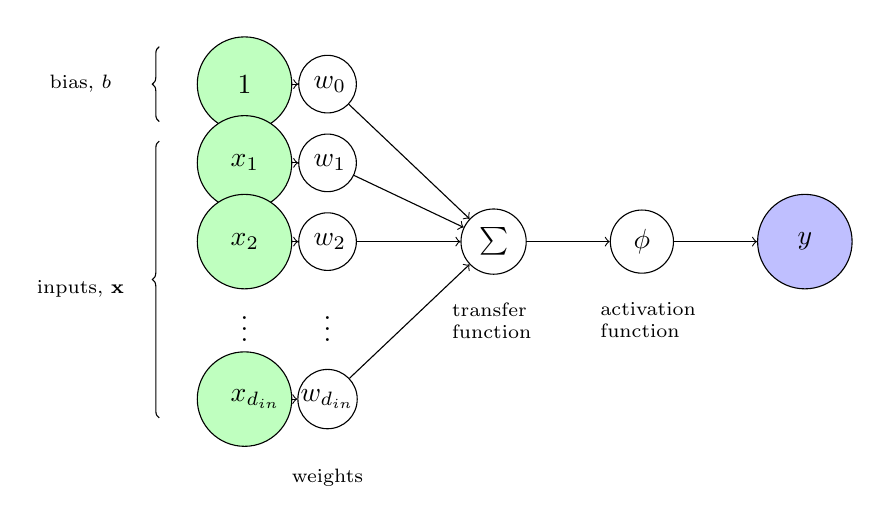
\begin{tikzpicture}
    \usetikzlibrary{decorations.pathreplacing}    % for TikZ braces
    \usetikzlibrary{positioning}                  % for TikZ relative positioning

    \node[function] at (\transferx, -{int(2)})  (transfer) {\transfersymbol};
    \node[function, right=3em of transfer] (activation) {\activationsymbol};
    \node[below of=activation,font=\scriptsize,text width=3em] {\activationlabel};
    \node[below of=transfer,font=\scriptsize,text width=3em] {\transferlabel};
    \node[output, right=\layersep of activation] (output) {\outputsymbol};
    \path[draw,->] (transfer) -- (activation);
    \path[draw,->] (activation) -- (output);

    % Iterate through each row of units.
    \foreach \n [evaluate=\n as \p using {int(\n-1)}] in {0,1,2,3,4} {
        \ifnum \n=0
        \node[input] at (0, -\n) (X-\n) {$1$};
        \node[weight] at (\layersep, -\n) (W-\n) {$w_\n$};
        \else \ifnum \n=3
        \node[] at (0, -\n) (X-\n) {$\vdots$};
        \node[] at (\layersep, -\n) (W-\n) {$\vdots$};
        \else \ifnum \n=4
        \node[input] at (0, -\n) (X-\n) {$x_{d_{{in}}}$};
        \node[weight,label={[xshift=-0.0em]center:$w_{d_{{in}}}$}] at (\layersep, -\n) (W-\n) {\phantom{$w_{d_{{in}}}$}};
        \else
        \node[input] at (0, -\n) (X-\n) {$x_\n$};
        \node[weight] at (\layersep, -\n) (W-\n) {$w_\n$};
        \fi
        \fi
        \fi

        % Arrow from input to weight.
        \ifnum \n=3
        \else
        \path[draw,->] (X-\n) -- (W-\n);
                    \path[draw,->] (W-\n) -- (transfer);
        \fi

    }

    % Brace for bias.
    \node[left=1em of X-0] (bias-brace) {};
    \node[above=1em of bias-brace] (bias-brace-up) {};
    \node[below=1em of bias-brace] (bias-brace-down) {};
    \draw[decorate,decoration = {brace}] (bias-brace-down) --  (bias-brace-up);
    \node[left of=bias-brace,font=\scriptsize] {bias, \biassymbol};

    % Brace for input.
    \node[below=10em of bias-brace-down] (input-brace-down) {};
    \node[below=5em of bias-brace-down] (input-brace) {};
    \draw[decorate,decoration = {brace}] (input-brace-down) --  (bias-brace-down);
    \node[left of=input-brace,font=\scriptsize] {inputs, \inputvecsymbol};

    % Weights label.
    \node[below of=W-4,font=\scriptsize] {\weightslabel};

\end{tikzpicture}

    \caption{Perceptron}
    \label{fig:perceptron}
\end{figure}

This mathematical mimicry of a biological neuron was first used used proposed by
Rosenblatt where a set of inputs $\mathbf{x}$ weighted using $\mathbf{w}$ before
being summed. If this sum surpassed a threshold, then a binary output of $1$ was
returned. \autoref{fig:perceptron} shows a more general formulation which
applies to the resulting field of deep learning, with any activation function
$\phi$ analogous for the level of excitation of a biological neuron in response
to its stimulus $\mathbf{x}$.

The primary criticism of the perceptron came in 1969 from Minsky and Papert
\cite{minsky69perceptrons}, where it was shown that the perceptron could only
solve \textit{linearly separable} functions, and failed to solve the XOR and
NXOR functions. They went on to claim that the research being done was doomed to
failure due to these limitations, resulting in little research in the area being
done until about the 1980's.

\subsection{Activation function}
%%%%%%%%%%%%%%%%%%%%%%%%%%%%%%%%%%%%%%%%%%%%%%%%%%%%%%%%%%%%%%%%%%%%%%%%%%%%%%%%

Since the early days of the perceptron, a wide variety of activation functions
$\phi$ have been used and improve upon the threshold step function.

%\begin{figure}[htbp]
%    \centering
%    \makeatletter
\pgfmathdeclarefunction{erf}{1}{%
    \begingroup
    \pgfmathparse{#1 > 0 ? 1 : -1}%
    \edef\sign{\pgfmathresult}%
    \pgfmathparse{abs(#1)}%
    \edef\x{\pgfmathresult}%
    \pgfmathparse{1/(1+0.3275911*\x)}%
    \edef\t{\pgfmathresult}%
    \pgfmathparse{%
        1 - (((((1.061405429*\t -1.453152027)*\t) + 1.421413741)*\t
        -0.284496736)*\t + 0.254829592)*\t*exp(-(\x*\x))}%
    \edef\y{\pgfmathresult}%
    \pgfmathparse{(\sign)*\y}%
    \pgfmath@smuggleone\pgfmathresult%
    \endgroup
}
%dep
%subfig
\begin{figure}[htp]
    \centering
    \captionsetup{format=hang} % hanging captions
    \subfloat[Threshold Step]{
        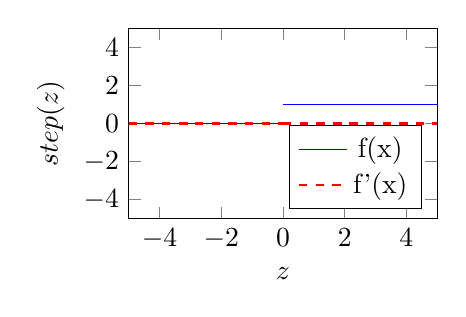
\begin{tikzpicture}
            \label{fig:threshold}
            \begin{axis}
                [width=5.5cm,height=4cm,ylabel=$step(z)$,xlabel=$z$,ymin=-5.0,ymax=5.0,xmin=-5,xmax=5,
                legend style={at={(0.95,0.05)},anchor=south east},]
                \addplot[blue,smooth, domain=-5:0] {0};
                \addplot[red,dashed, thick, domain=-5:0] {0};
                \addplot[blue,smooth, domain=-0:5] {1};
                \addplot[red,dashed, thick, domain=-0:5] {0};
                \addlegendentry{f(x)}
                \addlegendentry{f'(x)}
            \end{axis}
        \end{tikzpicture}
    }
    \subfloat[Linear]{
        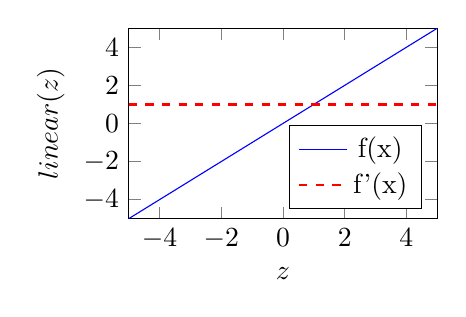
\begin{tikzpicture}
            \label{fig:linear}
            \begin{axis}
                [width=5.5cm,height=4cm,ylabel=$linear(z)$,xlabel=$z$,ymin=-5.0,ymax=5.0,xmin=-5,xmax=5,
                legend style={at={(0.95,0.05)},anchor=south east},]
                \addplot[blue,smooth] {x};
                \addlegendentry{f(x)}
                \addplot[red,dashed, thick] {1};
                \addlegendentry{f'(x)}
            \end{axis}
        \end{tikzpicture}
    }
    \subfloat[Sigmoid]{
        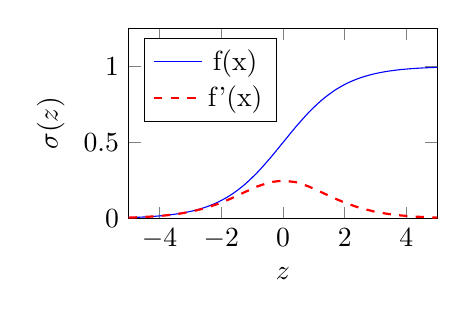
\begin{tikzpicture}
            \label{fig:sigmoid}
            \begin{axis}
                [width=5.5cm,height=4cm,ylabel=$\sigma(z)$,xlabel=$z$,ymin=0,ymax=1.25,xmin=-5,xmax=5,
                legend style={at={(0.05,0.95)},anchor=north west},]
                \addplot[blue,smooth] {1/(1+exp(-x))};
                \addlegendentry{f(x)}
                \addplot[red, dashed, thick] {1/(1+exp(-x)) * (1-1/(1+exp(-x)))};
                \addlegendentry{f'(x)}
            \end{axis}
        \end{tikzpicture}
    }\\
    \subfloat[Hyperbolic tangent]{
        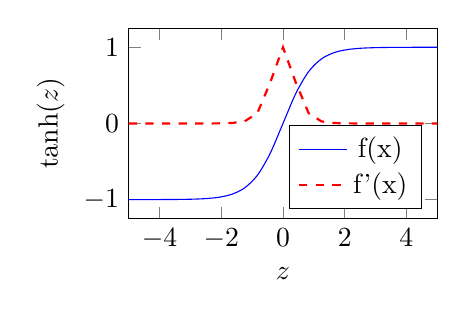
\begin{tikzpicture}
            \label{fig:hyperbolic_tangent}
            \begin{axis}
                [width=5.5cm,height=4cm,ylabel=$\tanh(z)$,xlabel=$z$,ymin=-1.25,ymax=1.25,xmin=-5,xmax=5, legend style={at={(0.95,0.05)},anchor=south east},]
                \addplot[blue,smooth] {tanh(x)};
                \addlegendentry{f(x)}
                \addplot[red,dashed, thick] {1/cosh(2*x)*1/cosh(2*x)};
                \addlegendentry{f'(x)}
            \end{axis}
        \end{tikzpicture}
    }
    \subfloat[ReLU]{
        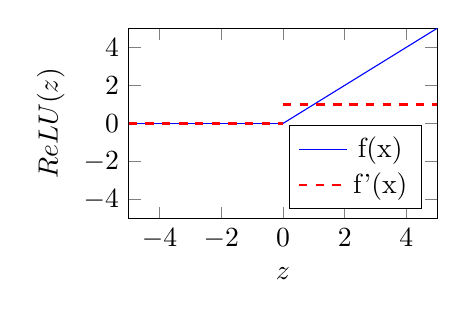
\begin{tikzpicture}
            \label{fig:relu}
            \begin{axis}
                [width=5.5cm,height=4cm,ylabel=$ReLU(z)$,xlabel=$z$,ymin=-5.0,ymax=5.0,xmin=-5,xmax=5,
                legend style={at={(0.95,0.05)},anchor=south east},]
                \addplot[blue,smooth, domain=-5:0] {0};
                \addplot[red,dashed, thick, domain=-5:0] {0};
                \addplot[blue,smooth, domain=-0:5] {x};
                \addplot[red,dashed, thick, domain=-0:5] {1};
                \addlegendentry{f(x)}
                \addlegendentry{f'(x)}
            \end{axis}
        \end{tikzpicture}
    }
    \subfloat[Leaky ReLU]{
        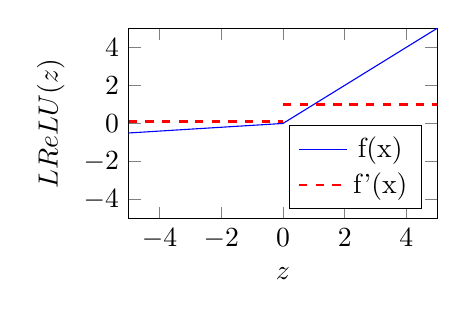
\begin{tikzpicture}
            \label{fig:lrelu}
            \begin{axis}
                [width=5.5cm,height=4cm,ylabel=$LReLU(z)$,xlabel=$z$,ymin=-5.0,ymax=5.0,xmin=-5,xmax=5,
                legend style={at={(0.95,0.05)},anchor=south east},]
                \addplot[blue,smooth, domain=-5:0] {0.1*x};
                \addplot[red,dashed, thick, domain=-5:0] {0.1};
                \addplot[blue,smooth, domain=-0:5] {x};
                \addplot[red,dashed, thick, domain=-0:5] {1};
                \addlegendentry{f(x)}
                \addlegendentry{f'(x)}
            \end{axis}
        \end{tikzpicture}
    }\\
    \subfloat[GELU]{
        \begin{tikzpicture}
            \label{fig:gelu}
            \begin{axis}
                [width=5.5cm,height=4cm,ylabel=$GELU(z)$,xlabel=$z$,ymin=-5.0,ymax=5.0,xmin=-5,xmax=5,
                legend style={at={(0.95,0.05)},anchor=south east},]
                \addplot[blue,smooth] {x * 0.5 * (1 + erf(x /sqrt(2)))};
                \addplot[red,dashed, thick] {0.5 * (1 + erf(x /sqrt(2))) + 1/sqrt(2*pi) * (exp(-x*x/2))};
                \addlegendentry{f(x)}
                \addlegendentry{f'(x)}
            \end{axis}
        \end{tikzpicture}
    }
    \subfloat[Swish]{
        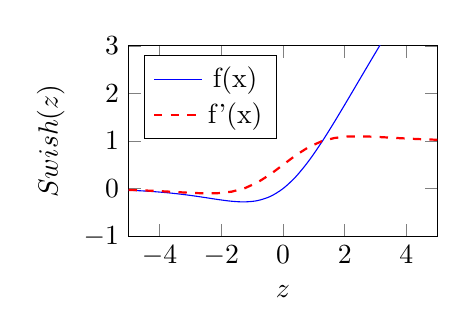
\begin{tikzpicture}
            \label{fig:swish}
            \begin{axis}
                [width=5.5cm,height=4cm,ylabel=$Swish(z)$,xlabel=$z$,ymin=-1,ymax=3.0,xmin=-5,xmax=5,
                legend style={at={(0.05,0.95)},anchor=north west},]
                \addplot[blue,smooth] {x*(1/(1+exp(-x)))}; % f (x) + σ (x) (1 − f (x))
                \addlegendentry{f(x)}
                \addplot[red, dashed, thick] {x/(1+exp(-x)) + 1/(1+exp(-x)) * (1-x/(1+exp(-x)))};
                \addlegendentry{f'(x)}
            \end{axis}
        \end{tikzpicture}
    }
    \subfloat[SIREN]{
        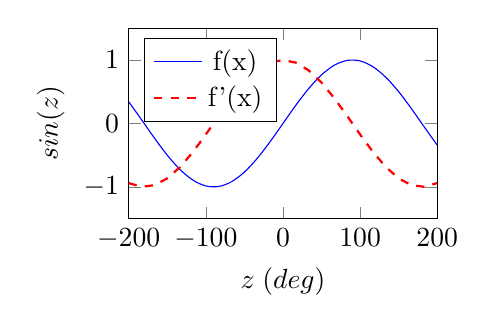
\begin{tikzpicture}
            \label{fig:siren}
            \begin{axis}
                [width=5.5cm,height=4cm,ylabel=$sin(z)$,xlabel=$z\;\text{(deg)}$,ymin=-1.5,ymax=1.5,xmin=-200,xmax=200,
                legend style={at={(0.05,0.95)},anchor=north west},]
                \addplot[blue,smooth,domain=-200:200] {sin(x)}; % f (x) + σ (x) (1 − f (x))
                \addlegendentry{f(x)}
                \addplot[red, dashed, thick,domain=-200:200] {cos(x)};
                \addlegendentry{f'(x)}
            \end{axis}
        \end{tikzpicture}
    }
    \caption[Activation functions.]{\textbf{Activation functions} used in \gls{DL}, included for results in their performance or historic significance in the applications of artificial neural networks.}
    \label{fig:activation-functions}
\end{figure}
%    \caption{Activation functions}
%    \label{fig:activation}
%\end{figure}
\makeatletter
\pgfmathdeclarefunction{erf}{1}{%
    \begingroup
    \pgfmathparse{#1 > 0 ? 1 : -1}%
    \edef\sign{\pgfmathresult}%
    \pgfmathparse{abs(#1)}%
    \edef\x{\pgfmathresult}%
    \pgfmathparse{1/(1+0.3275911*\x)}%
    \edef\t{\pgfmathresult}%
    \pgfmathparse{%
        1 - (((((1.061405429*\t -1.453152027)*\t) + 1.421413741)*\t
        -0.284496736)*\t + 0.254829592)*\t*exp(-(\x*\x))}%
    \edef\y{\pgfmathresult}%
    \pgfmathparse{(\sign)*\y}%
    \pgfmath@smuggleone\pgfmathresult%
    \endgroup
}
%dep
%subfig
\begin{figure}[htp]
    \centering
    \captionsetup{format=hang} % hanging captions
    \subfloat[Threshold Step]{
        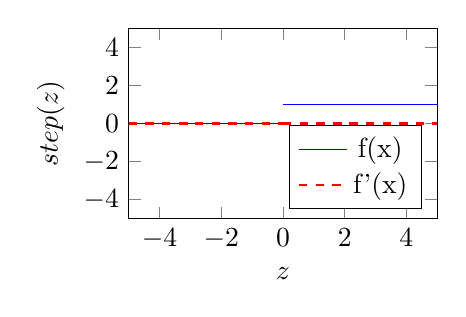
\begin{tikzpicture}
            \label{fig:threshold}
            \begin{axis}
                [width=5.5cm,height=4cm,ylabel=$step(z)$,xlabel=$z$,ymin=-5.0,ymax=5.0,xmin=-5,xmax=5,
                legend style={at={(0.95,0.05)},anchor=south east},]
                \addplot[blue,smooth, domain=-5:0] {0};
                \addplot[red,dashed, thick, domain=-5:0] {0};
                \addplot[blue,smooth, domain=-0:5] {1};
                \addplot[red,dashed, thick, domain=-0:5] {0};
                \addlegendentry{f(x)}
                \addlegendentry{f'(x)}
            \end{axis}
        \end{tikzpicture}
    }
    \subfloat[Linear]{
        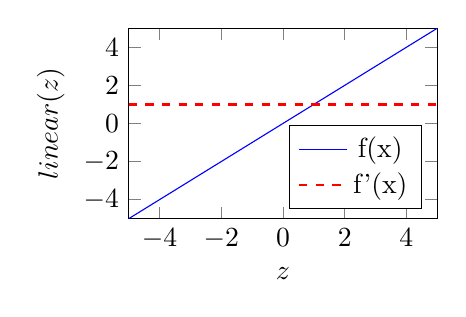
\begin{tikzpicture}
            \label{fig:linear}
            \begin{axis}
                [width=5.5cm,height=4cm,ylabel=$linear(z)$,xlabel=$z$,ymin=-5.0,ymax=5.0,xmin=-5,xmax=5,
                legend style={at={(0.95,0.05)},anchor=south east},]
                \addplot[blue,smooth] {x};
                \addlegendentry{f(x)}
                \addplot[red,dashed, thick] {1};
                \addlegendentry{f'(x)}
            \end{axis}
        \end{tikzpicture}
    }
    \subfloat[Sigmoid]{
        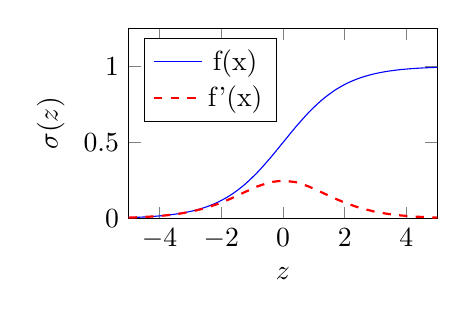
\begin{tikzpicture}
            \label{fig:sigmoid}
            \begin{axis}
                [width=5.5cm,height=4cm,ylabel=$\sigma(z)$,xlabel=$z$,ymin=0,ymax=1.25,xmin=-5,xmax=5,
                legend style={at={(0.05,0.95)},anchor=north west},]
                \addplot[blue,smooth] {1/(1+exp(-x))};
                \addlegendentry{f(x)}
                \addplot[red, dashed, thick] {1/(1+exp(-x)) * (1-1/(1+exp(-x)))};
                \addlegendentry{f'(x)}
            \end{axis}
        \end{tikzpicture}
    }\\
    \subfloat[Hyperbolic tangent]{
        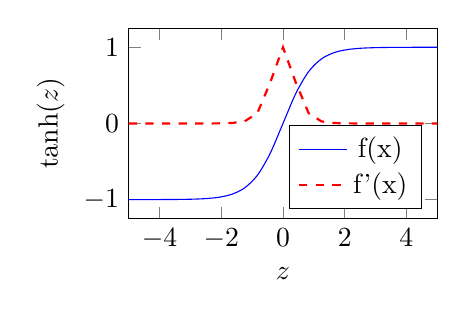
\begin{tikzpicture}
            \label{fig:hyperbolic_tangent}
            \begin{axis}
                [width=5.5cm,height=4cm,ylabel=$\tanh(z)$,xlabel=$z$,ymin=-1.25,ymax=1.25,xmin=-5,xmax=5, legend style={at={(0.95,0.05)},anchor=south east},]
                \addplot[blue,smooth] {tanh(x)};
                \addlegendentry{f(x)}
                \addplot[red,dashed, thick] {1/cosh(2*x)*1/cosh(2*x)};
                \addlegendentry{f'(x)}
            \end{axis}
        \end{tikzpicture}
    }
    \subfloat[ReLU]{
        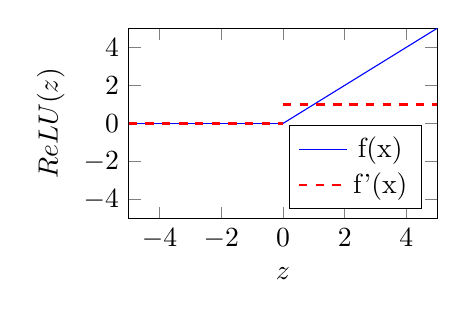
\begin{tikzpicture}
            \label{fig:relu}
            \begin{axis}
                [width=5.5cm,height=4cm,ylabel=$ReLU(z)$,xlabel=$z$,ymin=-5.0,ymax=5.0,xmin=-5,xmax=5,
                legend style={at={(0.95,0.05)},anchor=south east},]
                \addplot[blue,smooth, domain=-5:0] {0};
                \addplot[red,dashed, thick, domain=-5:0] {0};
                \addplot[blue,smooth, domain=-0:5] {x};
                \addplot[red,dashed, thick, domain=-0:5] {1};
                \addlegendentry{f(x)}
                \addlegendentry{f'(x)}
            \end{axis}
        \end{tikzpicture}
    }
    \subfloat[Leaky ReLU]{
        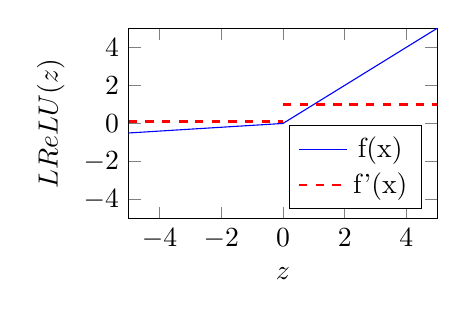
\begin{tikzpicture}
            \label{fig:lrelu}
            \begin{axis}
                [width=5.5cm,height=4cm,ylabel=$LReLU(z)$,xlabel=$z$,ymin=-5.0,ymax=5.0,xmin=-5,xmax=5,
                legend style={at={(0.95,0.05)},anchor=south east},]
                \addplot[blue,smooth, domain=-5:0] {0.1*x};
                \addplot[red,dashed, thick, domain=-5:0] {0.1};
                \addplot[blue,smooth, domain=-0:5] {x};
                \addplot[red,dashed, thick, domain=-0:5] {1};
                \addlegendentry{f(x)}
                \addlegendentry{f'(x)}
            \end{axis}
        \end{tikzpicture}
    }\\
    \subfloat[GELU]{
        \begin{tikzpicture}
            \label{fig:gelu}
            \begin{axis}
                [width=5.5cm,height=4cm,ylabel=$GELU(z)$,xlabel=$z$,ymin=-5.0,ymax=5.0,xmin=-5,xmax=5,
                legend style={at={(0.95,0.05)},anchor=south east},]
                \addplot[blue,smooth] {x * 0.5 * (1 + erf(x /sqrt(2)))};
                \addplot[red,dashed, thick] {0.5 * (1 + erf(x /sqrt(2))) + 1/sqrt(2*pi) * (exp(-x*x/2))};
                \addlegendentry{f(x)}
                \addlegendentry{f'(x)}
            \end{axis}
        \end{tikzpicture}
    }
    \subfloat[Swish]{
        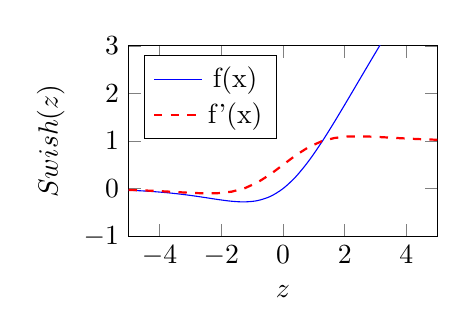
\begin{tikzpicture}
            \label{fig:swish}
            \begin{axis}
                [width=5.5cm,height=4cm,ylabel=$Swish(z)$,xlabel=$z$,ymin=-1,ymax=3.0,xmin=-5,xmax=5,
                legend style={at={(0.05,0.95)},anchor=north west},]
                \addplot[blue,smooth] {x*(1/(1+exp(-x)))}; % f (x) + σ (x) (1 − f (x))
                \addlegendentry{f(x)}
                \addplot[red, dashed, thick] {x/(1+exp(-x)) + 1/(1+exp(-x)) * (1-x/(1+exp(-x)))};
                \addlegendentry{f'(x)}
            \end{axis}
        \end{tikzpicture}
    }
    \subfloat[SIREN]{
        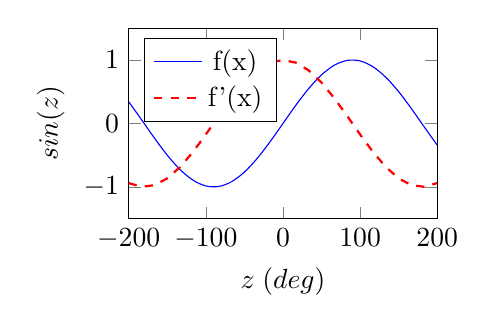
\begin{tikzpicture}
            \label{fig:siren}
            \begin{axis}
                [width=5.5cm,height=4cm,ylabel=$sin(z)$,xlabel=$z\;\text{(deg)}$,ymin=-1.5,ymax=1.5,xmin=-200,xmax=200,
                legend style={at={(0.05,0.95)},anchor=north west},]
                \addplot[blue,smooth,domain=-200:200] {sin(x)}; % f (x) + σ (x) (1 − f (x))
                \addlegendentry{f(x)}
                \addplot[red, dashed, thick,domain=-200:200] {cos(x)};
                \addlegendentry{f'(x)}
            \end{axis}
        \end{tikzpicture}
    }
    \caption[Activation functions.]{\textbf{Activation functions} used in \gls{DL}, included for results in their performance or historic significance in the applications of artificial neural networks.}
    \label{fig:activation-functions}
\end{figure}

\subsection{Multilayer perceptrons, a.k.a feed forward networks}
%%%%%%%%%%%%%%%%%%%%%%%%%%%%%%%%%%%%%%%%%%%%%%%%%%%%%%%%%%%%%%%%%%%%%%%%%%%%%%%%

$f(\mathbf{x};\mathbf{w}, b)=\mathbf{x}^T\mathbf{w}+b$; $x\in\mathbb{R}^{d_{in}}$, $\mathbf{w}\in\mathbb{R}^{d_{in}\times}$, $b\in\mathbb{R}^1$.

\begin{figure}
    \centering
    % MIT License
%
% Copyright (c) 2021 Geoffrey H. Garrett
%
% Permission is hereby granted, free of charge, to any person obtaining a copy
% of this software and associated documentation files (the "Software"), to deal
% in the Software without restriction, including without limitation the rights
% to use, copy, modify, merge, publish, distribute, sublicense, and/or sell
% copies of the Software, and to permit persons to whom the Software is
% furnished to do so, subject to the following conditions:
%
% The above copyright notice and this permission notice shall be included in all
% copies or substantial portions of the Software.
%
% THE SOFTWARE IS PROVIDED "AS IS", WITHOUT WARRANTY OF ANY KIND, EXPRESS OR
% IMPLIED, INCLUDING BUT NOT LIMITED TO THE WARRANTIES OF MERCHANTABILITY,
% FITNESS FOR A PARTICULAR PURPOSE AND NONINFRINGEMENT. IN NO EVENT SHALL THE
% AUTHORS OR COPYRIGHT HOLDERS BE LIABLE FOR ANY CLAIM, DAMAGES OR OTHER
% LIABILITY, WHETHER IN AN ACTION OF CONTRACT, TORT OR OTHERWISE, ARISING FROM,
% OUT OF OR IN CONNECTION WITH THE SOFTWARE OR THE USE OR OTHER DEALINGS IN THE
% SOFTWARE.

%%%%%%%%%%%%%%%%%%%%%%%%%%%%%%%%%%%%%%%%%%%%%%%%%%%%%%%%%%%%%%%%%%%%%%%%%%%%%%%
% ACKNOWLEDGEMENTS
%%%%%%%%%%%%%%%%%%%%%%%%%%%%%%%%%%%%%%%%%%%%%%%%%%%%%%%%%%%%%%%%%%%%%%%%%%%%%%%
% Adapted from:
% https://www.researchgate.net/figure/The-agent-environment-interaction-in-reinforcement-learning_fig1_328494763

%%%%%%%%%%%%%%%%%%%%%%%%%%%%%%%%%%%%%%%%%%%%%%%%%%%%%%%%%%%%%%%%%%%%%%%%%%%%%%%
% DEPENDENCIES
%%%%%%%%%%%%%%%%%%%%%%%%%%%%%%%%%%%%%%%%%%%%%%%%%%%%%%%%%%%%%%%%%%%%%%%%%%%%%%%
%\usepackage{tikz}
%\usetikzlibrary{decorations.pathreplacing}    % for TikZ braces
%\usetikzlibrary{positioning}                  % for TikZ relative positioning

%%%%%%%%%%%%%%%%%%%%%%%%%%%%%%%%%%%%%%%%%%%%%%%%%%%%%%%%%%%%%%%%%%%%%%%%%%%%%%%
% USER STYLING
%%%%%%%%%%%%%%%%%%%%%%%%%%%%%%%%%%%%%%%%%%%%%%%%%%%%%%%%%%%%%%%%%%%%%%%%%%%%%%%

% TikZ node design.
\tikzset{basic/.style={draw,text width=1em,text badly centered}}
\tikzset{input/.style={basic, fill=green!25, circle}}
\tikzset{output/.style={basic, fill=blue!25, circle}}
\tikzset{weight/.style={basic,circle}}
\tikzset{hidden/.style={basic,circle}}
\tikzset{function/.style={basic,circle}}
\def\layersep{3em}
\def\transferx{9em}
\def\hiddenx{7em}
\def\hiddenxn{12em}


\def\sep{4em}
\def\L{\gls{L}}       % number of hidden layers
\def\y{\gls{y_true}}  % output vector
\def\x{\gls{ml:x}}    % input vector
\def\h{\gls{a_vec}}   % hidden output
\def\nx{\gls{ml:n_x}}   % hidden output
\def\ny{\gls{ml:n_y}}   % hidden output


%%%%%%%%%%%%%%%%%%%%%%%%%%%%%%%%%%%%%%%%%%%%%%%%%%%%%%%%%%%%%%%%%%%%%%%%%%%%%%%
% TIKZ PICTURE
%%%%%%%%%%%%%%%%%%%%%%%%%%%%%%%%%%%%%%%%%%%%%%%%%%%%%%%%%%%%%%%%%%%%%%%%%%%%%%%
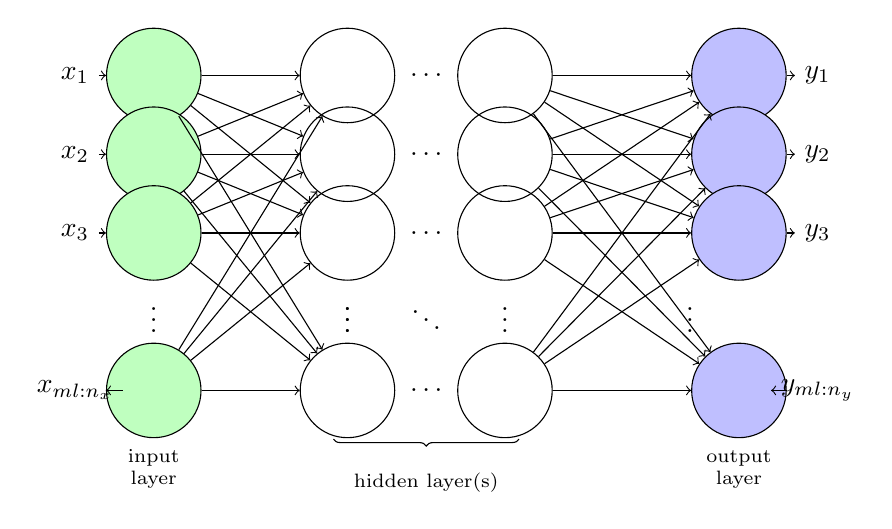
\begin{tikzpicture}
    \usetikzlibrary{decorations.pathreplacing}    % for TikZ braces
    \usetikzlibrary{positioning}                  % for TikZ relative positioning

    % input
    \foreach \n/\p in {0/1,1/2,2/3,3/4,4/5} {
        \ifnum \n=3
            % dots layer
            \node[] at (0, -\n) (X_\n) {$\vdots$};
            \node[] at (\hiddenx, -\n) (H1_\n) {$\vdots$};
            \node[right of=H1_\n] (M-\n) {$\ddots$};
            \node[below of=H1_2] (H2_\n) {$\vdots$};
            \node[below of=H2_2] (H2_\n) {$\vdots$};
            \node[right=5.7em of H2_\n] (Y_\n) {$\vdots$};
        \else
        \ifnum \n=4
            % n layer
            \node[input] at (0, -\n) (X_\n) {};
            \node[left of=X_\n] (I_\n) {$x_{\nx}$};
            \path[draw,->] (I_\n) -- (X_\n);
            \node[hidden] at (\hiddenx, -\n) (H1_\n) {}; %{$h_{n, 1}$};
            \node[right of= H1_\n] (M-\n) {$\ldots$};
            \node[hidden, right of= M-\n] (H2_\n) {}; % {$h_{n, m}$};
            \node[output, right= 5em of H2_\n] (Y_\n) {}; % {$h_{n, m}$};
            \node[right of=Y_\n] (O_\n) {$y_{\ny}$};
            \path[draw,->] (Y_\n) -- (O_\n);
        \else
            \node[input] at (0, -{\n}) (X_\n) {};
            \node[left of=X_\n] (I_\n) {$x_{\p}$};
            \path[draw,->] (I_\n) -- (X_\n);
            \node[hidden] at (\hiddenx, -\n) (H1_\n) {};%{$h_{\n, 1}$};
            \node[right of=H1_\n] (M-\n) {$\ldots$};
            \node[hidden, right of=M-\n] (H2_\n) {};% {$h_{\n, m}$};
            \node[output, right= 5em of H2_\n] (Y_\n) {}; % {$h_{n, m}$};
            \node[right of=Y_\n] (O_\n) {$y_\p$};
            \path[draw,->] (Y_\n) -- (O_\n);
        \fi
        \fi
    }

    % input layer connected to first hidden layer
    \foreach \j in {0,1,2,4} {
        \foreach \n in {0,1,2,4} {
            \path[draw,->] (X_\n) -- (H1_\j);
        }
    }

    % second hidden layer connected to output layer
    \foreach \j in {0,1,2,4} {
        \foreach \n in {0,1,2,4} {
            \path[draw,->] (H2_\n) -- (Y_\j);
        }
    }

    % labels
    \node[below of=X_4,font=\scriptsize, align=center] {input\\layer};
    \node[below of=Y_4,font=\scriptsize, align=center] {output\\layer};

    % brace for hidden layers
    \node[below=1em of M-4] (hidden-brace) {};
    \node[right=3em of hidden-brace] (hidden-brace-right) {};
    \node[left=3em of hidden-brace] (hidden-brace-left) {};
    \draw [decorate,decoration = {brace}] (hidden-brace-right) --  (hidden-brace-left);
    \node[below=0.5em of hidden-brace,font=\scriptsize] (hlayer) {hidden layer(s)};

\end{tikzpicture}


    \caption{Multilayer perceptron}
    \label{fig:mlp}
\end{figure}


\begin{figure}
    \centering
    % MIT License
%
% Copyright (c) 2021 Geoffrey H. Garrett
%
% Permission is hereby granted, free of charge, to any person obtaining a copy
% of this software and associated documentation files (the "Software"), to deal
% in the Software without restriction, including without limitation the rights
% to use, copy, modify, merge, publish, distribute, sublicense, and/or sell
% copies of the Software, and to permit persons to whom the Software is
% furnished to do so, subject to the following conditions:
%
% The above copyright notice and this permission notice shall be included in all
% copies or substantial portions of the Software.
%
% THE SOFTWARE IS PROVIDED "AS IS", WITHOUT WARRANTY OF ANY KIND, EXPRESS OR
% IMPLIED, INCLUDING BUT NOT LIMITED TO THE WARRANTIES OF MERCHANTABILITY,
% FITNESS FOR A PARTICULAR PURPOSE AND NONINFRINGEMENT. IN NO EVENT SHALL THE
% AUTHORS OR COPYRIGHT HOLDERS BE LIABLE FOR ANY CLAIM, DAMAGES OR OTHER
% LIABILITY, WHETHER IN AN ACTION OF CONTRACT, TORT OR OTHERWISE, ARISING FROM,
% OUT OF OR IN CONNECTION WITH THE SOFTWARE OR THE USE OR OTHER DEALINGS IN THE
% SOFTWARE.

%%%%%%%%%%%%%%%%%%%%%%%%%%%%%%%%%%%%%%%%%%%%%%%%%%%%%%%%%%%%%%%%%%%%%%%%%%%%%%%
% DEPENDENCIES
%%%%%%%%%%%%%%%%%%%%%%%%%%%%%%%%%%%%%%%%%%%%%%%%%%%%%%%%%%%%%%%%%%%%%%%%%%%%%%%
%\usepackage{tikz}
%\usetikzlibrary{decorations.pathreplacing}    % for TikZ braces
%\usetikzlibrary{positioning}                  % for TikZ relative positioning

%%%%%%%%%%%%%%%%%%%%%%%%%%%%%%%%%%%%%%%%%%%%%%%%%%%%%%%%%%%%%%%%%%%%%%%%%%%%%%%
% USER STYLING
%%%%%%%%%%%%%%%%%%%%%%%%%%%%%%%%%%%%%%%%%%%%%%%%%%%%%%%%%%%%%%%%%%%%%%%%%%%%%%%

% TikZ node design.
\tikzset{basic/.style={draw,text badly centered}}
\tikzset{input/.style={basic,minimum width=1.2cm, fill=green!25, circle}}
\tikzset{output/.style={basic,minimum width=1.2cm, fill=blue!25, circle}}
\tikzset{weight/.style={basic,circle}}
\tikzset{hidden/.style={basic,circle, minimum width=1.2cm}}
\tikzset{function/.style={basic,circle}}

\def\sep{4em}
\def\L{\gls{L}}       % number of hidden layers
\def\y{\gls{y_pred}}  % output vector
\def\x{\gls{ml:x}}    % input vector
\def\h{\gls{a_vec}}   % hidden output

%%%%%%%%%%%%%%%%%%%%%%%%%%%%%%%%%%%%%%%%%%%%%%%%%%%%%%%%%%%%%%%%%%%%%%%%%%%%%%%
% TIKZ PICTURE
%%%%%%%%%%%%%%%%%%%%%%%%%%%%%%%%%%%%%%%%%%%%%%%%%%%%%%%%%%%%%%%%%%%%%%%%%%%%%%%
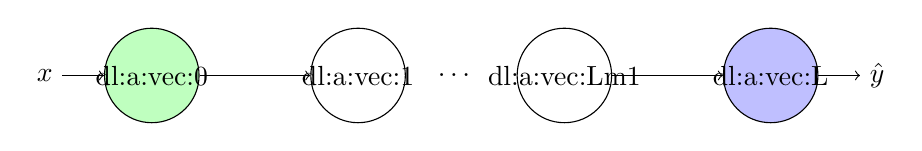
\begin{tikzpicture}
    \node[input, label={[xshift=-0.0em]center:\gls{dl:a:vec:0}}] (X) {\phantom{\gls{dl:a:vec:1}}};
    \node[, left=1.5em of X] (in) {$\bm{x}$};

    \node[hidden, right=\sep of X, label={[xshift=-0.0em]center:\gls{dl:a:vec:1}}] (H1) {\phantom{\gls{dl:a:vec:1}}};
    \node[hidden, right=\sep of H1, label={[xshift=-0.0em]center:\gls{dl:a:vec:Lm1}}] (H2) {\phantom{\gls{dl:a:vec:Lm1}}};
    \node[output, right=\sep of H2,  label={[xshift=-0.0em]center:\gls{dl:a:vec:L}}] (Y) {\phantom{\gls{dl:a:vec:L}}};
    \node[, right=1.5em of Y] (out) {$\bm{\hat{y}}$};

    \path[draw,->] (in) -- (X);
    \path[draw,->] (X) -- (H1);
    \node[right=0.8em of H1] (M) {$\ldots$};
    \path[draw,->] (H2) -- (Y);
    \path[draw,->] (Y) -- (out);
\end{tikzpicture}


    \caption{Multilayer perceptron}
    \label{fig:mlp-vec}
\end{figure}


\begin{equation}
    \mathbf{h}^{(1)} = g^{(1)} \bigg(\mathbf{W}^{{(1)}\;T}\mathbf{x} + \mathbf{b}^{(1)}\bigg);
\end{equation}

\begin{equation}
    \mathbf{h}^{(2)} = g^{(2)} \bigg(\mathbf{W}^{{(2)}\;T}\mathbf{h}^{(1)} + \mathbf{b}^{(2)}\bigg);
\end{equation}

\subsection{Gradient based learning}
%%%%%%%%%%%%%%%%%%%%%%%%%%%%%%%%%%%%%%%%%%%%%%%%%%%%%%%%%%%%%%%%%%%%%%%%%%%%%%%%

\subsection{Universal Approximation Properties and Depth}
%%%%%%%%%%%%%%%%%%%%%%%%%%%%%%%%%%%%%%%%%%%%%%%%%%%%%%%%%%%%%%%%%%%%%%%%%%%%%%%%

A linear model by definition, may only optimised to represent linear functions.
It has advantages in its simplicity to optimise however we often require our
estimator models to learn nonlinear functions.

\subsection{Backpropagation}
%%%%%%%%%%%%%%%%%%%%%%%%%%%%%%%%%%%%%%%%%%%%%%%%%%%%%%%%%%%%%%%%%%%%%%%%%%%%%%%%

Backpropagation, short for "backward propagation of errors," is a
\textit{supervised learning} algorithm for artificial neural networks using
\textit{gradient descent}.


\section{Reinforcement Learning\label{ssec:RL}}
%%%%%%%%%%%%%%%%%%%%%%%%%%%%%%%%%%%%%%%%%%%%%%%%%%%%%%%%%%%%%%%%%%%%%%%%%%%%%%%%

\tikzset{basic/.style={draw,text width=1em,text badly centered}}
\tikzset{component/.style={rectangle, draw=black, thick, text width=7em,align=center, rounded corners, minimum height=2em}}

\begin{figure}[!htp]
    \centering
    \captionsetup{format=hang} % hanging captions

    \tikzstyle{block} = [rectangle, draw,
    text width=8em, text centered, rounded corners, minimum height=4em]

    \tikzstyle{line} = [draw, -latex]

    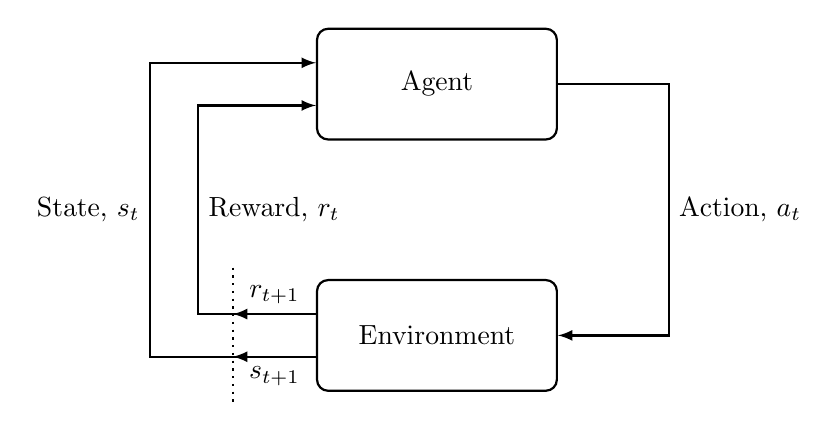
\begin{tikzpicture}[node distance = 6em, auto, thick]
        \node [block] (Agent) {Agent};
        \node [block, below=5em of Agent] (Environment) {Environment};
        \node [left=3em of Environment] (Dashed) {};
        \node [above=1.7em of Dashed] (Dashed-up) {};
        \node [below=1.7em of Dashed] (Dashed-down) {};

        \path [line] (Agent.0) --++ (4em,0em) |- node [near start]{Action, $a_t$} (Environment.0);

        \path [line] (Environment.190) -- (Environment.190-|Dashed-down.east) node [midway, label={[xshift=-0.0em]center:$s_{t+1}$}] {\phantom{$s_{t+1}$}};
        \path [line] (Environment.170) -- (Environment.170-|Dashed-up.east) node [midway, above, label={[xshift=-0.0em]center:$r_{t+1}$}] {\phantom{$r_{t+1}$}};

        \path [line] (Environment.190|-Environment.190) --++ (-6em,0em) |- node [near start] {} node [near start, label={[xshift=-0.0em]center:State, $s_t$}] {\phantom{State, $s_t$}} (Agent.170);
        \path [line] (Environment.170|-Environment.170) --++ (-4.25em,0em) |- node [near start, right] {} node [near start, right, label={[xshift=-0.0em]center:Reward, $r_t$}] {\phantom{Reward, $r_t$}} (Agent.190);

        \draw[dotted] (Dashed-up.east) -- (Dashed-down.east);


    \end{tikzpicture}
    \caption{\textbf{The agent-environment interaction interface} illustrates the interaction between an agent and its environment. The agent takes an action $a_t$ and receives a reward $r_{t+1}$ and a new state $s_{t+1}$, subject to the environment's dynamics.}
    \label{fig:agent-environment}

\end{figure}

\begin{itemize}
    \item states and observations,
    \item action spaces,
    \item policies,
    \item trajectories,
    \item different formulations of return,
    \item the RL optimization problem,
    \item and value functions.
\end{itemize}

\subsection{Taxonomy of Reinforcement Learning}
%%%%%%%%%%%%%%%%%%%%%%%%%%%%%%%%%%%%%%%%%%%%%%%%%%%%%%%%%%%%%%%%%%%%%%%%%%%%%%%%

\subsection{Value-based methods}
%%%%%%%%%%%%%%%%%%%%%%%%%%%%%%%%%%%%%%%%%%%%%%%%%%%%%%%%%%%%%%%%%%%%%%%%%%%%%%%%

\subsection{Policy-based methods}
%%%%%%%%%%%%%%%%%%%%%%%%%%%%%%%%%%%%%%%%%%%%%%%%%%%%%%%%%%%%%%%%%%%%%%%%%%%%%%%%

\subsection{Policy gradient}
%%%%%%%%%%%%%%%%%%%%%%%%%%%%%%%%%%%%%%%%%%%%%%%%%%%%%%%%%%%%%%%%%%%%%%%%%%%%%%%%

\subsection{Deep deterministic policy gradient (DDPG)}
%%%%%%%%%%%%%%%%%%%%%%%%%%%%%%%%%%%%%%%%%%%%%%%%%%%%%%%%%%%%%%%%%%%%%%%%%%%%%%%%
